%% In the documentclass line, replace "noanswers" with "answers" to view the key.

\documentclass[noanswers]{exam}
\usepackage[utf8]{inputenc}

\title{Practice Problems}
\author{Chapter 4}
\date{STAT 3090}

\usepackage[bottom=2.2cm, left=2.2cm, right=2.2cm, top=2.2cm]{geometry}
%\usepackage[paperheight=11in, paperwidth=17in, margin=1in]{geometry}
\usepackage{dsfont}
\usepackage{amsmath}
\usepackage{amssymb}
\usepackage{amsthm}
\usepackage{array}
\usepackage{stmaryrd}
\usepackage{pgfplots}
\pgfplotsset{width=10cm,compat=1.9}
\usepackage{multicol}
\setlength{\columnsep}{1in}
\usepackage{nicefrac}

\usepackage{multirow}
\usepackage{enumitem}[shortlabels]
\usepackage{tabu}
\definecolor{purp}{RGB}{102,0,204}
\usepackage{tabularx}
\newcolumntype{C}{>{\centering\arraybackslash $}X<{$}}
\usepackage{wrapfig}
\usepackage[export]{adjustbox}


\makeatletter
\pagestyle{headandfoot}
\firstpageheader{\@date}{\@title}{\@author}
\firstpageheadrule
\runningfootrule
\runningfooter{}{\thepage\ / \numpages}{\@title}
\makeatother

\newcommand{\abs}[1]{\left|#1\right|}
\newcommand{\mat}[4]{\left( \begin{tabular}{>{$}c<{$} >{$}c<{$}} #1&#2 \\ #3&#4 \end{tabular} \right)}
\newcommand{\msc}[1]{\mathds{#1}}
\newcommand{\Z}{\mathds{Z}}
\newcommand{\R}{\mathds{R}}
\newcommand{\N}{\mathds{N}}
\newcommand{\Q}{\mathds{Q}}
\newcommand{\C}{\mathds{C}}
\newcommand{\so}{\implies}
\newcommand{\set}[2]{\left\{ #1 \:|\: #2 \right\}}
\newcommand{\bso}{\Longleftarrow}
\newcommand{\ra}{\rightarrow}
\newcommand{\gen}[1]{\left\langle #1 \right\rangle}
\newcommand{\olin}[1]{\overline{#1}}
\newcommand{\Img}[1]{\text{Im}\left(#1\right)}
\newcommand{\llra}{\longleftrightarrow}
\newcommand{\lra}{\longrightarrow}
\newcommand{\xra}[1]{\xrightarrow{#1}}
\newcommand{\wo}{\setminus}
\newcommand{\mcal}[1]{\mathcal{#1}}
\newcommand{\Aut}[1]{\text{Aut}\left(#1\right)}
\newcommand{\Inn}[1]{\text{Inn}\left(#1\right)}
\newcommand{\syl}[2]{\text{Syl}_{#1}(#2)}
\newcommand{\norm}[1]{\left\|#1\right\|}
\newcommand{\infnorm}[1]{\left\|#1\right\|_{\infty}}
\newcommand{\xn}{\{x_n\}}
\newcommand{\sig}{\sigma}
\newcommand{\id}{\text{id}}
\newcommand{\ep}{\epsilon}
\newcommand{\st}{\text{ s.t. }}
\newcommand{\ran}[1]{\text{Ran}(#1)}
\newcommand{\nCr}[2]{\binom{#1}{#2}}
\newcommand{\Exr}[1]{\paragraph{Exercise #1:}}
\newcommand{\pg}{\paragraph{}}
\newcommand{\ulin}[1]{\underline{#1}}
\newcommand{\tc}[1]{\textcolor{purp}{#1}}

% Solution Specs
\unframedsolutions
\renewcommand{\solutiontitle}{}
\SolutionEmphasis{\color{purp}}
\CorrectChoiceEmphasis{\color{purp}\bfseries}

%\begin{solution}[\stretch{1}]
%	hurp durp flurp
%\end{solution}

%\pagestyle{empty}

\begin{document}

%\noindent\begin{tabular}{@{}p{.3in}p{3in}@{}}
%Name: & \hrulefill
%\end{tabular}
%
%\vspace{2mm}
%
%\noindent\begin{tabular}{@{}p{1.05in}p{3.2in}@{}}
%Group Members: & \hrulefill
%\end{tabular}

\begin{questions} 
	
	\question A data set has a mean that is much higher than the median. Which of the following is most likely \textbf{true}?
	
	\vspace{2mm}
	
	\begin{choices}
	
		\choice The distribution of values is symmetric.
		\choice The distribution of values is skewed left.
		\CorrectChoice The distribution of values is skewed right.
		\choice The distribution has a few high outliers.	
	
	\end{choices}
	
	\vspace{3mm}
	
	\question The Clemson intramural basketball team has 15 players who are each a different height. The team trades its shortest player for a tall center who is now the tallest person on the team. Which of the statements is \textbf{false}?
	
	\vspace{2mm}
	
	\begin{choices}
	
		\choice The range of heights might be different.
		\CorrectChoice The median height will remain the same.
		\choice The mean height of the team will increase.
		\choice The standard deviation of the heights might be different.	
	
	\end{choices}
	
	\vspace{3mm}
	
	\question \textbf{Explain} your reasoning for your answer to Question 2. Why did you choose your answer over the others?
	
	\begin{solution}[\stretch{1}]
	
			\vspace{3mm}		
		
			Student answers will vary. Correct answers should include something about how the median will shift positions when the lowest observation is removed and a high observation is added.

			\vspace{3mm}		
			
		\end{solution}
		
	\question At Hogwarts, Professor Slughorn's Potions class of 23 students had an average of 82 on their last exam. Professor Snape's class of 27 students had an average of 77 on the same test. What is the average of the two classes combined? (Hint: Use a weighted average.)
	
	\begin{solution}[\stretch{1}]
	
	\vspace{3mm}
	
	$\displaystyle \overline{x}=\frac{23(82)+27(77)}{23+27}=\frac{3965}{50}=79.3$
	
	\vspace{3mm}
	
	\end{solution}
	
	\question In Jane Austen's nineteenth century English literature class, attendance counts for 5\% of the final grade, quizzes count for 15\%, exams count for 45\%, and the final exam counts for 35\%. Jane has averages of 95 for attendance, 92 for quizzes, and 85 for exams. What would she need to score on the final to have an A (a course average of 90) in the course?
	
	\begin{solution}[\stretch{1}]
	
			\vspace{3mm}
			
			$0.05(95)+0.15(92)+0.45(85)+0.35x=90$
			
			\vspace{3mm}
			
			$0.35x=33.2$

			\vspace{3mm}	
			
			$x=94.86$	
			
		\end{solution}
		
	\newpage
	
	\question At an Amateur Rubik's Cube Competition, the solving times (in seconds) for each of ten randomly-selected participants are listed in the table below. 
	
	\begin{center}
    \begin{tabular}{| c | c | c | c | c |}
        \hline
        28 & 32 & 33 & 35 & 37 \\
        \hline
        39 & 42 & 46 & 51 & 59 \\
        \hline 
    \end{tabular}
\end{center}

Find the following statistics from your sample. For each one, be sure to \textbf{label} the values with the appropriate symbol, \textbf{show} your work, and include your \textbf{answer} with \textbf{units}.

\vspace{3mm}

\begin{parts}
	
	\part Calculate the \textbf{mean} of the distribution.
	
	\begin{solution}[\stretch{1}]
	
	\vspace{3mm}
	
	$\displaystyle \overline{x}=\frac{28+32+33+...+59}{10}=\frac{402}{10}=40.2$ seconds
	
	\vspace{3mm}
	
	\end{solution}
	
	\part Find the \textbf{median} of the distribution.
	
	\begin{solution}[\stretch{1}]
	
	\vspace{3mm}
	
	$n=10$ is even, so we average the $\frac{n}{2}=5$th and 6th values.
	
	\vspace{3mm}
	
	Median $=\displaystyle \frac{37+39}{2}=38$ seconds
	
	\vspace{3mm}
	
	\end{solution}
	
	\part Find the \textbf{standard deviation} of the distribution. (Hint: Take the variance first.)
	
	\begin{solution}[\stretch{1}]
	
	\vspace{3mm}
	
	Formula 4.4: $\displaystyle s^2=\frac{\sum{(x-\overline{x})^2}}{n-1}=\frac{(28-40.2)^2+(32-40.2)^2+\dots+(59-40.2)^2}{10-1}=\frac{813.6}{9}=90.4$ sec$^2$
	
	\vspace{3mm}
	
	Formula 4.5: $\displaystyle s^2=\frac{\sum x_i^2-\frac{(\sum x_i)^2}{n}}{n-1}=\frac{16,974-\frac{(402)^2}{10}}{9}=90.4$ sec$^2$
	
	\vspace{3mm}
	
	$s=\sqrt{90.4}\approx 9.51$ seconds
	
	\vspace{3mm}
	
	\end{solution}
	
\end{parts}

%	\question A company that produces longboard wheels wants to get an estimate of how many of the wheel bearings it produces on a given day are defective. The resident statistician at the company counts the number of defective bearings produced each day in the month of January. Her results are summarized below.
%	
%	\begin{center}
%    \begin{tabular}{| c | c | }
%        \hline
%        \textbf{Defect Count} & \textbf{Frequency} \\ 
%        \hline
%        0 & 10\\
%        \hline
%        1 & 8\\   
%        \hline
%        2 & 7\\
%        \hline
%        3 & 3\\   
%        \hline
%        4 & 1\\
%        \hline
%        5 & 2\\   
%        \hline
%    \end{tabular}
%\end{center}
%
%\begin{parts}
%	\part What is the \textbf{mean} number of defective bearings produced each day by the company? Show your work.
%	
%	\begin{solution}[\stretch{1}]
%	
%	\vspace{3mm}
%	
%	$\overline{x}=\frac{0(10)+1(8)+2(7)+...+5(2)}{31}=\frac{45}{31}=1.45$ defects per day
%	
%	\vspace{3mm}
%	
%	\end{solution}
%	
%	\part What is the \textbf{median} number of defective bearings per day?
%	
%	\begin{solution}[\stretch{1}]
%	
%	\vspace{3mm}
%	
%	Since there are 31 observations, the median will be $16^{\text{th}}$ observation. The $16^{\text{th}}$ observation falls in the second row.
%
%\vspace{3mm}
%
%Median $=1$ defect per day
%	
%	\vspace{3mm}
%	
%	\end{solution}
%	
%\end{parts}
%	

\newpage

	\question The number of coffee shop customers on a given day at Central Perk follows a distribution that is roughly symmetric and unimodal with a mean of 240 customers and a standard deviation of 20 customers.

\vspace{3mm}	
	
	\begin{parts}
	
	\part Why is it appropriate to use the Empirical Rule here? \mbox{(Hint: What do we know about the distribution?)}
	\begin{solution}[\stretch{1}]
	
		
			The distribution is symmetric and unimodal (bell-shaped), so the Empirical Rule applies.

			\vspace{3mm}		
			
		\end{solution}
	
	\part According to the Empirical Rule, on what percentage of days can the coffee shop expect between 220 and 280 customers? Draw a \textbf{sketch} of the distribution with axis values and appropriate shading.
	
	\begin{solution}[\stretch{1}]
		
	\vspace{3mm}	
		
				\begin{center}
    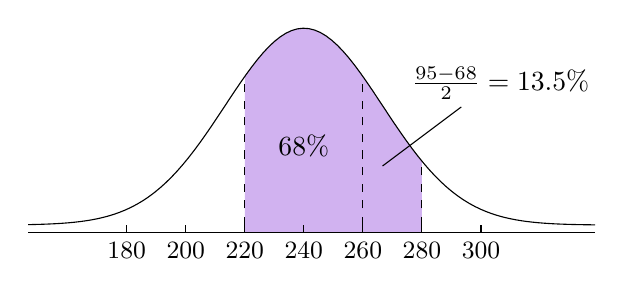
\begin{tikzpicture}
        \def\normaltwo{\x,{2.5*1/exp(((\x-3)^2)/2)}}
        \def\mu{3}
        \def\y{5}
        \def\x{1}
        \def\fy{2.5*1/exp(((\y-3)^2)/2)}
        \def\fx{2.5*1/exp(((\x-3)^2)/2)}
        \fill [fill=purp!30] ({2.25},-.1) -- plot[domain={2.25}:{4.5}] (\normaltwo) -- ({4.5},-.1) -- cycle;
        \draw[domain=-.5:6.7,samples=100] plot (\normaltwo) node[right] {};
        \draw[] ({\mu},{0}) -- ({\mu},-.1) node[below] {\small{$240$}};
        
        
        % Tick Marks for One Std Dev
        \draw[] ({3.75},{0}) -- ({3.75},-.1) node[below] {\small{$260 $}};
        \draw[] ({2.25},{0}) -- ({2.25},-.1) node[below] {\small{$220 $}};
        \draw[] ({1.5},{0}) -- ({1.5},-.1) node[below] {\small{$200 $}};
        \draw[] ({.75},{0}) -- ({.75},-.1) node[below] {\small{$180 $}};
        \draw[] ({4.5},{0}) -- ({4.5},-.1) node[below] {\small{$280$}};
        \draw[] ({5.25},{0}) -- ({5.25},-.1) node[below] {\small{$300$}};
        
        \draw[dashed] (2.25,0) -- (2.25,1.8) {};
        \draw[dashed] (3.75,0) -- (3.75,1.8) {};
        \draw[dashed] (4.5,0) -- (4.5,.75) {};
        
        \draw[-] (-.5,-.1) -- (6.7,-.1) node[right] {};  
        
        \node[] at (3,1) {68\%};
        \draw[-] (4,.75) -- (5,1.5);
        \node[] at (5.5,1.8) {$\frac{95-68}{2}=13.5\%$};
        
               
%        \node[] at (6.5, 2) {$68 + \frac{95-68}{2}=81.5\%$};
%        \draw[-] (5,1.7) -- (3.5,1);
    \end{tikzpicture}
    \end{center}
    
    \vspace{3mm}
    
    Central Perk can expect between 220 and 280 customers on \underline{81.5\% of days}.
		
		\vspace{3mm}
	\end{solution}
	
	\part The maximum occupancy of the coffee shop is 300 customers. According to the Empirical Rule, on what percentage of days can the coffee shop expect more than 300 customers, having to turn people away? Draw a \textbf{sketch} with axis values and appropriate shading.
	
	\begin{solution}[\stretch{1}]
	
	\vspace{3mm}
		
				\begin{center}
    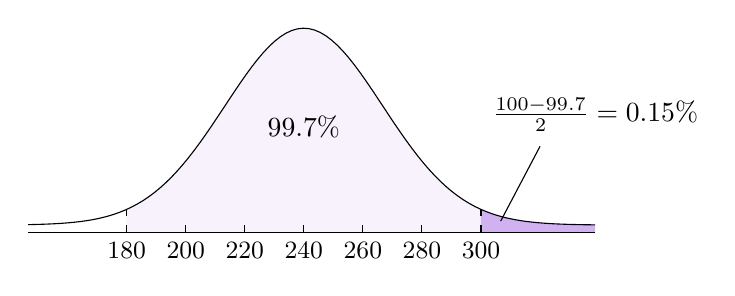
\begin{tikzpicture}
        \def\normaltwo{\x,{2.5*1/exp(((\x-3)^2)/2)}}
        \def\mu{3}
        \def\y{5}
        \def\x{1}
        \def\fy{2.5*1/exp(((\y-3)^2)/2)}
        \def\fx{2.5*1/exp(((\x-3)^2)/2)}
        \fill [fill=purp!5] ({.75},-.1) -- plot[domain={.75}:{5.25}] (\normaltwo) -- ({5.25},-.1) -- cycle;
        \fill [fill=purp!30] ({5.25},-.1) -- plot[domain={5.25}:{6.7}] (\normaltwo) -- ({6.7},-.1) -- cycle;
        \draw[domain=-.5:6.7,samples=100] plot (\normaltwo) node[right] {};
        \draw[] ({\mu},{0}) -- ({\mu},-.1) node[below] {\small{$240$}};
        
        % Tick Marks for One Std Dev
        \draw[] ({3.75},{0}) -- ({3.75},-.1) node[below] {\small{$260 $}};
        \draw[] ({2.25},{0}) -- ({2.25},-.1) node[below] {\small{$220 $}};
        \draw[] ({1.5},{0}) -- ({1.5},-.1) node[below] {\small{$200 $}};
        \draw[] ({.75},{0}) -- ({.75},-.1) node[below] {\small{$180 $}};
        \draw[] ({4.5},{0}) -- ({4.5},-.1) node[below] {\small{$280$}};
        \draw[] ({5.25},{0}) -- ({5.25},-.1) node[below] {\small{$300$}};
        
%        \draw[dashed] (\mu,0) -- (\mu,2.5) {};
        
        % Number Line
        \draw[-] (-.5,-.1) -- (6.7,-.1) node[right] {};         
        
        \draw[dashed] (.75,-.1) -- (.75,.2) {};
        \draw[dashed] (5.25,-.1) -- (5.25,.2) {};
        
        \node[] at (3, 1.25) {99.7\%};
        
        \node[] at (6.7, 1.4) {$\frac{100-99.7}{2}=0.15\%$};
        \draw[-] (5.5,.05) -- (6,1);
    \end{tikzpicture}
    \end{center}
    
    \vspace{3mm}
    
    We would only expect the coffee shop to have to turn customers away on \underline{0.15\% of days}.
		
	\end{solution}
	
	\end{parts}
	
	
	\question Suppose we didn't know that the distribution above was symmetric and unimodal, so we had to use \mbox{Chebyshev's} Rule to learn about our data.
	
	\vspace{3mm}
	
	\begin{parts}
		\part On at least what percent of days should we expect between 200 and 280 customers? (Hint: First identify $k$, the number of standard deviations from the mean, to use in Formula 4.9.) Show your work!
		
		\begin{solution}[\stretch{1}]
		
		\vspace{3mm}
		
		$k=2 \; \Rightarrow \; 1-\frac{1}{2^2}=\frac{3}{4}=0.75$
		
		\vspace{2mm}
		
		Central Perk can expect between 200 and 280 customers on \underline{at least 75\% of days}.
		
		\vspace{3mm}
		
		\end{solution}
		
		\part Determine the range of the number of customers Central Perk can expect on at least 55.6\% of days.
				
		\begin{solution}[\stretch{1}]
		
		\vspace{3mm}
		
		Solve $1-\frac{1}{k^2}=0.556$ for $k$. $\Rightarrow k\approx 1.5$
		
		\vspace{2mm}
		
		At least 55.6\% of days will have between $240-1.5(20)=\underline{210}$ and $240+1.5(20)=\underline{270}$ customers.
		
		\end{solution}
		
	\end{parts}

\newpage 

	\question The following list represents the times, in minutes, that it took 10 randomly-selected fishermen at Issaqueena Lake to get the first bite on their hook.
\begin{center}
    3, 19, 21, 21, 23, 25, 28, 30, 31, 32
\end{center}
	
	\vspace{3mm}
	
	\begin{parts}
	
	\part Write the \textbf{five-number summary} for the data. Label the values and show any calculations.
	
	\begin{solution}[\stretch{1}]
	
			\vspace{3mm}		
		
			Min $=3$, $Q_1=21$, $M=\frac{23+25}{2}=24$, $Q_3=30$, Max $=32$

			\vspace{3mm}		
			
		\end{solution}
		
		\part Calculate the \textbf{fences} and state whether there are any \textbf{outliers}.
	
	\begin{solution}[\stretch{1}]
			
			\vspace{3mm}		
		
			Lower Fence: $Q_1-1.5(IQR)=21-1.5(9)=7.5 \; \Rightarrow \; 3$ is a low outlier.

\vspace{3mm}

Upper Fence: $Q_3+1.5(IQR)=30+1.5(9)=43.5 \; \Rightarrow \;$ No high outliers.

			\vspace{3mm}	
			
		\end{solution}
	
	\part Construct a \textbf{boxplot}. Include a title with units for your horizontal axis.
	
	\begin{solution}[\stretch{2}]
	
			\vspace{3mm}		
		
		\begin{center}
			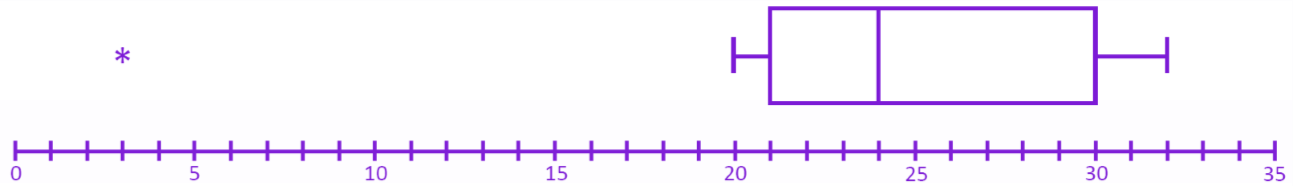
\includegraphics[scale=.7]{STAT_3090_Ch4_boxplot.png}
			\end{center} 
			\vspace{3mm}		
			
		\end{solution}
		
		\part Describe the \textbf{distribution} of the boxplot you constructed by discussing its shape, center, spread, and any outliers.
		
		\begin{solution}[\stretch{1}]
	
			\vspace{3mm}		
		
			The distribution of bite times is skewed left with one low outlier of 3 minutes. It has a median of 24 minutes and an IQR of 9 minutes.
			
			\vspace{3mm}		
			
		\end{solution}
		
	\end{parts}


\end{questions}

%-----------------------------------------------------------------------------%

\end{document}
